\documentclass[twoside]{book}

% Packages required by doxygen
\usepackage{calc}
\usepackage{doxygen}
\usepackage{graphicx}
\usepackage[utf8]{inputenc}
\usepackage{makeidx}
\usepackage{multicol}
\usepackage{multirow}
\usepackage{textcomp}
\usepackage[table]{xcolor}

% Font selection
\usepackage[T1]{fontenc}
\usepackage{mathptmx}
\usepackage[scaled=.90]{helvet}
\usepackage{courier}
\usepackage{amssymb}
\usepackage{sectsty}
\renewcommand{\familydefault}{\sfdefault}
\allsectionsfont{%
  \fontseries{bc}\selectfont%
  \color{darkgray}%
}
\renewcommand{\DoxyLabelFont}{%
  \fontseries{bc}\selectfont%
  \color{darkgray}%
}

% Page & text layout
\usepackage{geometry}
\geometry{%
  a4paper,%
  top=2.5cm,%
  bottom=2.5cm,%
  left=2.5cm,%
  right=2.5cm%
}
\tolerance=750
\hfuzz=15pt
\hbadness=750
\setlength{\emergencystretch}{15pt}
\setlength{\parindent}{0cm}
\setlength{\parskip}{0.2cm}
\makeatletter
\renewcommand{\paragraph}{%
  \@startsection{paragraph}{4}{0ex}{-1.0ex}{1.0ex}{%
    \normalfont\normalsize\bfseries\SS@parafont%
  }%
}
\renewcommand{\subparagraph}{%
  \@startsection{subparagraph}{5}{0ex}{-1.0ex}{1.0ex}{%
    \normalfont\normalsize\bfseries\SS@subparafont%
  }%
}
\makeatother

% Headers & footers
\usepackage{fancyhdr}
\pagestyle{fancyplain}
\fancyhead[LE]{\fancyplain{}{\bfseries\thepage}}
\fancyhead[CE]{\fancyplain{}{}}
\fancyhead[RE]{\fancyplain{}{\bfseries\leftmark}}
\fancyhead[LO]{\fancyplain{}{\bfseries\rightmark}}
\fancyhead[CO]{\fancyplain{}{}}
\fancyhead[RO]{\fancyplain{}{\bfseries\thepage}}
\fancyfoot[LE]{\fancyplain{}{}}
\fancyfoot[CE]{\fancyplain{}{}}
\fancyfoot[RE]{\fancyplain{}{\bfseries\scriptsize Generated on Fri May 8 2015 13\-:02\-:54 for Robot Simulator-\/ Iteration three by Doxygen }}
\fancyfoot[LO]{\fancyplain{}{\bfseries\scriptsize Generated on Fri May 8 2015 13\-:02\-:54 for Robot Simulator-\/ Iteration three by Doxygen }}
\fancyfoot[CO]{\fancyplain{}{}}
\fancyfoot[RO]{\fancyplain{}{}}
\renewcommand{\footrulewidth}{0.4pt}
\renewcommand{\chaptermark}[1]{%
  \markboth{#1}{}%
}
\renewcommand{\sectionmark}[1]{%
  \markright{\thesection\ #1}%
}

% Indices & bibliography
\usepackage{natbib}
\usepackage[titles]{tocloft}
\setcounter{tocdepth}{3}
\setcounter{secnumdepth}{5}
\makeindex

% Hyperlinks (required, but should be loaded last)
\usepackage{ifpdf}
\ifpdf
  \usepackage[pdftex,pagebackref=true]{hyperref}
\else
  \usepackage[ps2pdf,pagebackref=true]{hyperref}
\fi
\hypersetup{%
  colorlinks=true,%
  linkcolor=blue,%
  citecolor=blue,%
  unicode%
}

% Custom commands
\newcommand{\clearemptydoublepage}{%
  \newpage{\pagestyle{empty}\cleardoublepage}%
}


%===== C O N T E N T S =====

\begin{document}

% Titlepage & ToC
\hypersetup{pageanchor=false}
\pagenumbering{roman}
\begin{titlepage}
\vspace*{7cm}
\begin{center}%
{\Large Robot Simulator-\/ Iteration three }\\
\vspace*{1cm}
{\large Generated by Doxygen 1.8.6}\\
\vspace*{0.5cm}
{\small Fri May 8 2015 13:02:54}\\
\end{center}
\end{titlepage}
\clearemptydoublepage
\tableofcontents
\clearemptydoublepage
\pagenumbering{arabic}
\hypersetup{pageanchor=true}

%--- Begin generated contents ---
\chapter{Slime Volleyball-\/ Individual Project Index Page}
\label{index}\hypertarget{index}{}\hypertarget{index_intro_sec}{}\section{Introduction}\label{index_intro_sec}
For my individual project, Professor Larson granted me permission to create a game called \hyperlink{classSlime}{Slime} Volleyball. \hyperlink{classSlime}{Slime} Volleyball adheres to some of the same rules as both pong and regular volleyball. Rules\-:
\begin{DoxyEnumerate}
\item A player gains a point when the ball lands on the opponents side of the net.
\item A player may hit the ball as many times as they would like.
\item A player may not leave their side of the court.
\item If the ball hits a wall or the side of the net it will bounce, therefore the ball cannot go out of bounds.
\item If the ball hits a player it will bounce and change direction depending on the balls velocity and the angle of the impact.
\item If the ball hits the bottom of a player it will be \char`\"{}spiked\char`\"{} and go in the the opposite direction.
\end{DoxyEnumerate}

The main classes in this program are\-: Environment -\/ The environment tracks what is going on inside the game and where all objects are. It is responsible for telling the slimes and the ball when to move as well as informing them if a collision occurred and how they are expected to react. \hyperlink{classSlime}{Slime} -\/ Slimes are the players in \hyperlink{classSlime}{Slime} Volleyball. They are human or ai controlled and move around the environment base on inputs which each reflect a direction. The valid inputs can cause a slime to move left, move right, jump or stop moving. As a human player, slimes can be controlled with the a,w,d keys if player1 or the arrow keys if player 2. \hyperlink{classBall}{Ball} -\/ The ball is a self updating object in \hyperlink{classSlime}{Slime} Volleyball that updates its position only based on the change in time given by the environment. However, the velocity can be changed by the environment if there is a collision with another object. \hyperlink{classObject}{Object} -\/ The overall class for in game items, both \hyperlink{classSlime}{Slime} and \hyperlink{classBall}{Ball} inherit from \hyperlink{classObject}{Object} so it has many basic functions.

Supporting Files\-: \hyperlink{classRenderEnv}{Render\-Env} -\/ A basic class which puts the Slimes and \hyperlink{classBall}{Ball} into the environment. Drawing -\/ Drawing is responsible for displaying all in game objects such as the Slimes,\hyperlink{classBall}{Ball} and net.

Author\-: Matthew Bullis

This project would not have been possible if my group for the previous iterations had not helped to build a solid base for this project.\-Alex Wang, Arun Parthiban, Aaron Switzer wrote many of the functions used in \hyperlink{classSlime}{Slime} Volleyball.\hypertarget{index_install_sec}{}\section{Installation}\label{index_install_sec}
To use this software, just run the given make file by typing \char`\"{}make\char`\"{}(without quotation marks) on the U\-N\-I\-X terminal while in the src directory. 
\chapter{Hierarchical Index}
\section{Class Hierarchy}
This inheritance list is sorted roughly, but not completely, alphabetically\-:\begin{DoxyCompactList}
\item \contentsline{section}{environment}{\pageref{classenvironment}}{}
\item \contentsline{section}{Object}{\pageref{classObject}}{}
\begin{DoxyCompactList}
\item \contentsline{section}{Ball}{\pageref{classBall}}{}
\item \contentsline{section}{Slime}{\pageref{classSlime}}{}
\end{DoxyCompactList}
\item \contentsline{section}{Position}{\pageref{structPosition}}{}
\item \contentsline{section}{Render\-Env}{\pageref{classRenderEnv}}{}
\item \contentsline{section}{Velocity}{\pageref{structVelocity}}{}
\end{DoxyCompactList}

\chapter{Class Index}
\section{Class List}
Here are the classes, structs, unions and interfaces with brief descriptions\-:\begin{DoxyCompactList}
\item\contentsline{section}{\hyperlink{classBall}{Ball} }{\pageref{classBall}}{}
\item\contentsline{section}{\hyperlink{classenvironment}{environment} }{\pageref{classenvironment}}{}
\item\contentsline{section}{\hyperlink{classObject}{Object} }{\pageref{classObject}}{}
\item\contentsline{section}{\hyperlink{structPosition}{Position} }{\pageref{structPosition}}{}
\item\contentsline{section}{\hyperlink{classRenderEnv}{Render\-Env} }{\pageref{classRenderEnv}}{}
\item\contentsline{section}{\hyperlink{classSlime}{Slime} }{\pageref{classSlime}}{}
\item\contentsline{section}{\hyperlink{structVelocity}{Velocity} }{\pageref{structVelocity}}{}
\end{DoxyCompactList}

\chapter{File Index}
\section{File List}
Here is a list of all documented files with brief descriptions\-:\begin{DoxyCompactList}
\item\contentsline{section}{{\bfseries Ball.\-h} }{\pageref{Ball_8h}}{}
\item\contentsline{section}{{\bfseries Documentation.\-h} }{\pageref{Documentation_8h}}{}
\item\contentsline{section}{\hyperlink{drawing_8cpp}{drawing.\-cpp} }{\pageref{drawing_8cpp}}{}
\item\contentsline{section}{{\bfseries drawing.\-h} }{\pageref{drawing_8h}}{}
\item\contentsline{section}{{\bfseries environment.\-h} }{\pageref{environment_8h}}{}
\item\contentsline{section}{{\bfseries Object.\-h} }{\pageref{Object_8h}}{}
\item\contentsline{section}{{\bfseries Render\-Env.\-h} }{\pageref{RenderEnv_8h}}{}
\item\contentsline{section}{{\bfseries Slime.\-h} }{\pageref{Slime_8h}}{}
\end{DoxyCompactList}

\chapter{Class Documentation}
\hypertarget{classBall}{\section{Ball Class Reference}
\label{classBall}\index{Ball@{Ball}}
}
Inheritance diagram for Ball\-:\begin{figure}[H]
\begin{center}
\leavevmode
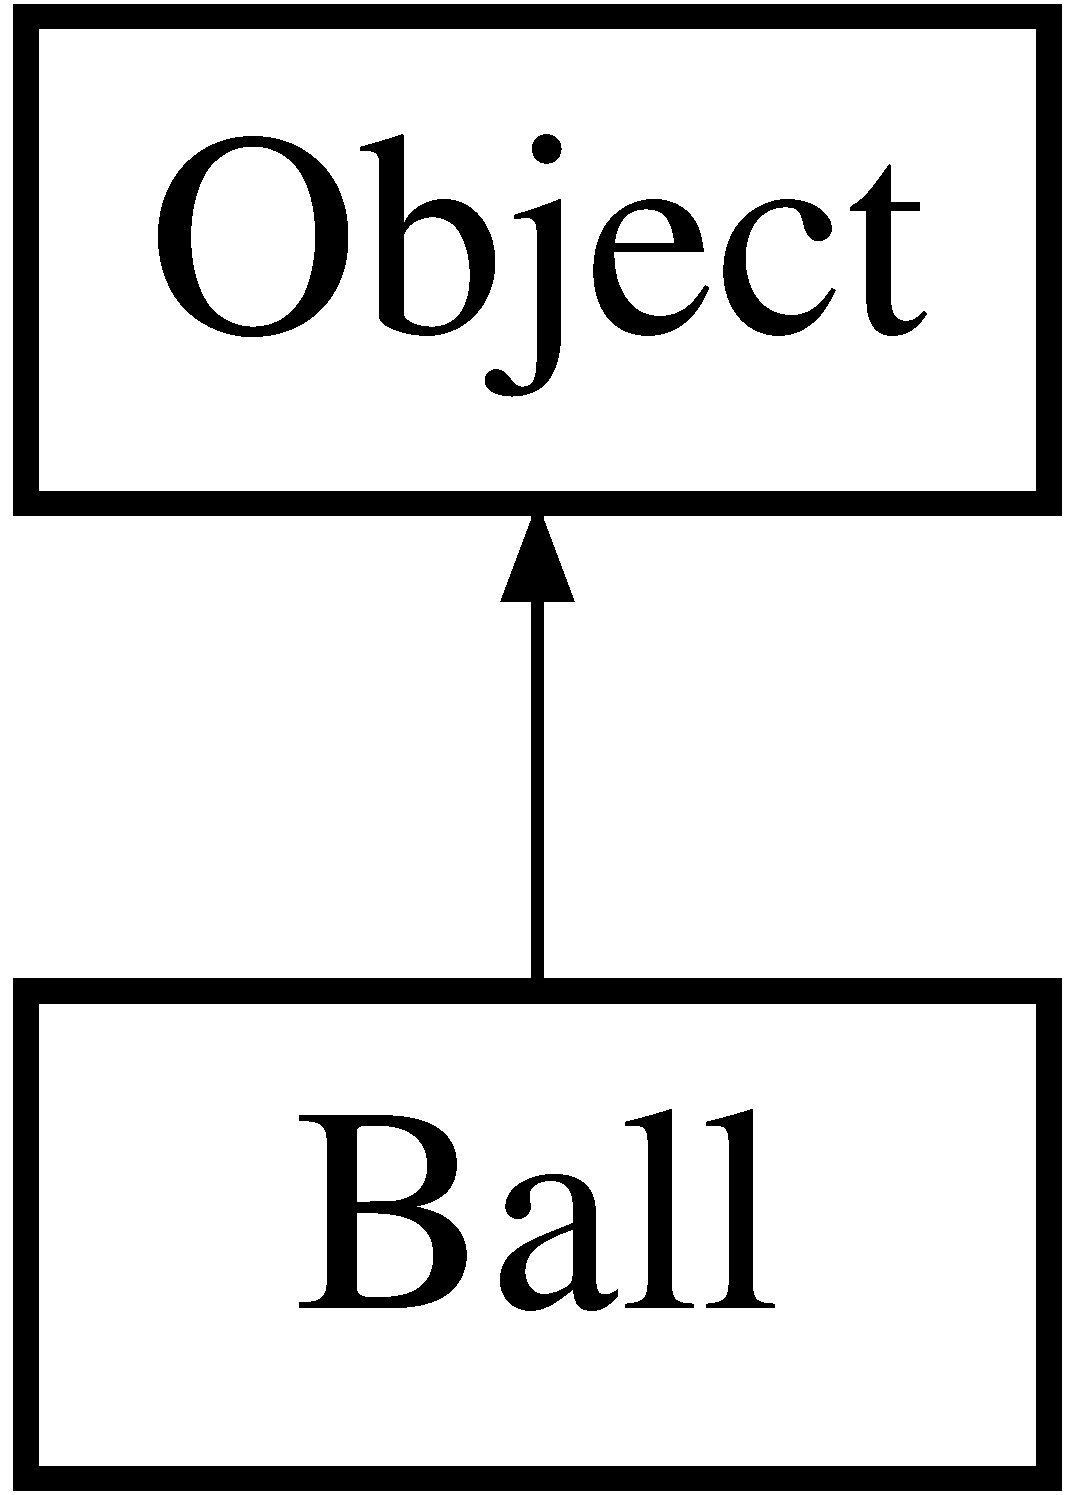
\includegraphics[height=2.000000cm]{classBall}
\end{center}
\end{figure}
\subsection*{Public Member Functions}
\begin{DoxyCompactItemize}
\item 
\hyperlink{classBall_a86a144d3dad6c953e422e32435923bbb}{Ball} ()
\item 
\hyperlink{classBall_a29d1cfd97f0bfddcbf86f5d71ed4a74a}{Ball} (int, int)
\item 
void \hyperlink{classBall_ae58dee698dec173afc66000b4660e949}{move} (int)
\item 
void \hyperlink{classBall_ac8bde2e98049adf194667e6a6505112d}{wallbounce} ()
\item 
void \hyperlink{classBall_a82ffc97c926776abe6f508eaa997214d}{bounce} (double, double)
\item 
\hyperlink{structPosition}{Position} \hyperlink{classBall_a77d822e70c4f55c2d0d514b76cb1330b}{get\-Landing\-Zone} ()
\item 
void \hyperlink{classBall_aa9efc8640cf5de6377caa0d64cc8fb13}{recalc\-Landing\-Zone} ()
\end{DoxyCompactItemize}
\subsection*{Static Public Attributes}
\begin{DoxyCompactItemize}
\item 
\hypertarget{classBall_af17d8911edff6e79ebf5c353d8643e00}{static const float {\bfseries gravity} = 0.\-9}\label{classBall_af17d8911edff6e79ebf5c353d8643e00}

\item 
\hypertarget{classBall_a24bf806a98565f572173378c74043f41}{static const int {\bfseries ball\-Speed} = 650}\label{classBall_a24bf806a98565f572173378c74043f41}

\item 
\hypertarget{classBall_a82712fef17d72513e4dd92dff79c9765}{static const int {\bfseries S\-C\-A\-L\-A\-R} = 1000}\label{classBall_a82712fef17d72513e4dd92dff79c9765}

\end{DoxyCompactItemize}
\subsection*{Additional Inherited Members}


\subsection{Constructor \& Destructor Documentation}
\hypertarget{classBall_a86a144d3dad6c953e422e32435923bbb}{\index{Ball@{Ball}!Ball@{Ball}}
\index{Ball@{Ball}!Ball@{Ball}}
\subsubsection[{Ball}]{\setlength{\rightskip}{0pt plus 5cm}Ball\-::\-Ball (
\begin{DoxyParamCaption}
{}
\end{DoxyParamCaption}
)}}\label{classBall_a86a144d3dad6c953e422e32435923bbb}
default constructor initializes all variables \begin{DoxyAuthor}{Author}
Matthew Bullis 
\end{DoxyAuthor}
\hypertarget{classBall_a29d1cfd97f0bfddcbf86f5d71ed4a74a}{\index{Ball@{Ball}!Ball@{Ball}}
\index{Ball@{Ball}!Ball@{Ball}}
\subsubsection[{Ball}]{\setlength{\rightskip}{0pt plus 5cm}Ball\-::\-Ball (
\begin{DoxyParamCaption}
\item[{int}]{xpos, }
\item[{int}]{ypos}
\end{DoxyParamCaption}
)}}\label{classBall_a29d1cfd97f0bfddcbf86f5d71ed4a74a}
Constructor with two passed parameters \begin{DoxyAuthor}{Author}
Matthew Bullis 
\end{DoxyAuthor}

\begin{DoxyParams}{Parameters}
{\em int} & xpos for x coordinate \\
\hline
{\em int} & ypos for y coordinate \\
\hline
\end{DoxyParams}


\subsection{Member Function Documentation}
\hypertarget{classBall_a82ffc97c926776abe6f508eaa997214d}{\index{Ball@{Ball}!bounce@{bounce}}
\index{bounce@{bounce}!Ball@{Ball}}
\subsubsection[{bounce}]{\setlength{\rightskip}{0pt plus 5cm}void Ball\-::bounce (
\begin{DoxyParamCaption}
\item[{double}]{nx, }
\item[{double}]{ny}
\end{DoxyParamCaption}
)}}\label{classBall_a82ffc97c926776abe6f508eaa997214d}
Updates the ball's velocity if there is a collision another object 
\begin{DoxyParams}{Parameters}
{\em double} & nx the x coordinate of the neutral vector between the ball and object \\
\hline
{\em double} & ny the y coordinate of the neutral vector between the ball and object \\
\hline
\end{DoxyParams}
\begin{DoxyAuthor}{Author}
Matthew Bullis 
\end{DoxyAuthor}
\hypertarget{classBall_a77d822e70c4f55c2d0d514b76cb1330b}{\index{Ball@{Ball}!get\-Landing\-Zone@{get\-Landing\-Zone}}
\index{get\-Landing\-Zone@{get\-Landing\-Zone}!Ball@{Ball}}
\subsubsection[{get\-Landing\-Zone}]{\setlength{\rightskip}{0pt plus 5cm}{\bf Position} Ball\-::get\-Landing\-Zone (
\begin{DoxyParamCaption}
{}
\end{DoxyParamCaption}
)}}\label{classBall_a77d822e70c4f55c2d0d514b76cb1330b}
Returns the position the ball will land at \begin{DoxyAuthor}{Author}
Matthew Bullis 
\end{DoxyAuthor}
\hypertarget{classBall_ae58dee698dec173afc66000b4660e949}{\index{Ball@{Ball}!move@{move}}
\index{move@{move}!Ball@{Ball}}
\subsubsection[{move}]{\setlength{\rightskip}{0pt plus 5cm}void Ball\-::move (
\begin{DoxyParamCaption}
\item[{int}]{time}
\end{DoxyParamCaption}
)}}\label{classBall_ae58dee698dec173afc66000b4660e949}
Updates the ball's travel position based on the time since last update 
\begin{DoxyParams}{Parameters}
{\em int} & time for the elapsed time \\
\hline
\end{DoxyParams}
\begin{DoxyAuthor}{Author}
Matthew Bullis 
\end{DoxyAuthor}
\hypertarget{classBall_aa9efc8640cf5de6377caa0d64cc8fb13}{\index{Ball@{Ball}!recalc\-Landing\-Zone@{recalc\-Landing\-Zone}}
\index{recalc\-Landing\-Zone@{recalc\-Landing\-Zone}!Ball@{Ball}}
\subsubsection[{recalc\-Landing\-Zone}]{\setlength{\rightskip}{0pt plus 5cm}void Ball\-::recalc\-Landing\-Zone (
\begin{DoxyParamCaption}
{}
\end{DoxyParamCaption}
)}}\label{classBall_aa9efc8640cf5de6377caa0d64cc8fb13}
Calculates where the ball will land using the balls current position and velocity \begin{DoxyAuthor}{Author}
Matthew Bullis 
\end{DoxyAuthor}
\hypertarget{classBall_ac8bde2e98049adf194667e6a6505112d}{\index{Ball@{Ball}!wallbounce@{wallbounce}}
\index{wallbounce@{wallbounce}!Ball@{Ball}}
\subsubsection[{wallbounce}]{\setlength{\rightskip}{0pt plus 5cm}void Ball\-::wallbounce (
\begin{DoxyParamCaption}
{}
\end{DoxyParamCaption}
)}}\label{classBall_ac8bde2e98049adf194667e6a6505112d}
Updates the ball's velocity if there is a collision with the wall \begin{DoxyAuthor}{Author}
Matthew Bullis 
\end{DoxyAuthor}


The documentation for this class was generated from the following files\-:\begin{DoxyCompactItemize}
\item 
Ball.\-h\item 
Ball.\-cpp\end{DoxyCompactItemize}

\hypertarget{classenvironment}{\section{environment Class Reference}
\label{classenvironment}\index{environment@{environment}}
}


{\ttfamily \#include $<$environment.\-h$>$}

\subsection*{Public Member Functions}
\begin{DoxyCompactItemize}
\item 
\hyperlink{classenvironment_aaff2c2f57d25e0af6981a673e0b85045}{environment} ()
\item 
void \hyperlink{classenvironment_acbd5c1e053c91847f7605cd8b29e7a10}{update} (int)
\item 
\hypertarget{classenvironment_ab8fa5dc66ae9a7cfd921f0097f6ff317}{void {\bfseries init} ()}\label{classenvironment_ab8fa5dc66ae9a7cfd921f0097f6ff317}

\item 
void \hyperlink{classenvironment_abfe6af8bba0929f848e73a0fa279fd1c}{add\-Ball} (int, int)
\item 
int \hyperlink{classenvironment_a4106cb73fcead35475ae8c33ffe89942}{get\-W\-I\-N\-D\-O\-W\-\_\-\-H\-E\-I\-G\-H\-T} ()
\item 
int \hyperlink{classenvironment_acb1222ce73320ac1aec5721f5c2783b6}{get\-W\-I\-N\-D\-O\-W\-\_\-\-W\-I\-D\-T\-H} ()
\item 
\hypertarget{classenvironment_a1f9d00c3197390de97d385e5871d92b2}{int {\bfseries get\-N\-E\-T\-\_\-\-H\-E\-I\-G\-H\-T} ()}\label{classenvironment_a1f9d00c3197390de97d385e5871d92b2}

\item 
void \hyperlink{classenvironment_a5e9a836194ff2b790e84a884d4dd09bf}{set\-W\-I\-N\-D\-O\-W\-\_\-\-H\-E\-I\-G\-H\-T} (int)
\item 
void \hyperlink{classenvironment_a64a6ec127866efa6a1e49e1700fea83b}{set\-W\-I\-N\-D\-O\-W\-\_\-\-W\-I\-D\-T\-H} (int)
\item 
void \hyperlink{classenvironment_a07df3c9f4baeecc67f94bd3eacf8e151}{register\-With} (\hyperlink{classSlime}{Slime}, bool)
\item 
void \hyperlink{classenvironment_acd0761acd4b21d3a49be966046af11cf}{register\-With} (\hyperlink{classBall}{Ball})
\item 
\hypertarget{classenvironment_a63d3437ab81498e7b884208f3f457711}{void {\bfseries score} (int)}\label{classenvironment_a63d3437ab81498e7b884208f3f457711}

\item 
\hypertarget{classenvironment_ada0be30d21ce8f4d621199c68d17612f}{void {\bfseries reset} (int)}\label{classenvironment_ada0be30d21ce8f4d621199c68d17612f}

\item 
\hypertarget{classenvironment_a50dbb74afc6b6bd9042379599cb01618}{void {\bfseries set\-Multiplayer} (bool)}\label{classenvironment_a50dbb74afc6b6bd9042379599cb01618}

\item 
\hypertarget{classenvironment_af5743bf8d1dcf909e95432651b53e89f}{bool {\bfseries is\-Multiplayer} ()}\label{classenvironment_af5743bf8d1dcf909e95432651b53e89f}

\end{DoxyCompactItemize}
\subsection*{Public Attributes}
\begin{DoxyCompactItemize}
\item 
\hypertarget{classenvironment_a40a78733acaf8f88ad526561e00c03f7}{\hyperlink{classSlime}{Slime} {\bfseries player1}}\label{classenvironment_a40a78733acaf8f88ad526561e00c03f7}

\item 
\hypertarget{classenvironment_a3ff6ba2d2f9d7ec5466e4139f478a835}{\hyperlink{classSlime}{Slime} {\bfseries player2}}\label{classenvironment_a3ff6ba2d2f9d7ec5466e4139f478a835}

\item 
\hypertarget{classenvironment_ac7e61528875363067f0ce8d1de440fa1}{\hyperlink{classBall}{Ball} {\bfseries ball}}\label{classenvironment_ac7e61528875363067f0ce8d1de440fa1}

\end{DoxyCompactItemize}


\subsection{Detailed Description}
Worked on by Arun Parthiban Additional implementation by Alex Wang 

\subsection{Constructor \& Destructor Documentation}
\hypertarget{classenvironment_aaff2c2f57d25e0af6981a673e0b85045}{\index{environment@{environment}!environment@{environment}}
\index{environment@{environment}!environment@{environment}}
\subsubsection[{environment}]{\setlength{\rightskip}{0pt plus 5cm}environment\-::environment (
\begin{DoxyParamCaption}
{}
\end{DoxyParamCaption}
)}}\label{classenvironment_aaff2c2f57d25e0af6981a673e0b85045}
default constructor initializes private variables \begin{DoxyAuthor}{Author}
Arun Parthiban 
\end{DoxyAuthor}


\subsection{Member Function Documentation}
\hypertarget{classenvironment_abfe6af8bba0929f848e73a0fa279fd1c}{\index{environment@{environment}!add\-Ball@{add\-Ball}}
\index{add\-Ball@{add\-Ball}!environment@{environment}}
\subsubsection[{add\-Ball}]{\setlength{\rightskip}{0pt plus 5cm}void environment\-::add\-Ball (
\begin{DoxyParamCaption}
\item[{int}]{x, }
\item[{int}]{y}
\end{DoxyParamCaption}
)}}\label{classenvironment_abfe6af8bba0929f848e73a0fa279fd1c}
Adds a \hyperlink{classBall}{Ball} to the environment, with given coordinates 
\begin{DoxyParams}{Parameters}
{\em x} & for x\-Position of \hyperlink{classBall}{Ball} \\
\hline
{\em y} & for y\-Position of \hyperlink{classBall}{Ball} \\
\hline
\end{DoxyParams}
\begin{DoxyAuthor}{Author}
Matthew Bullis 
\end{DoxyAuthor}
\hypertarget{classenvironment_a4106cb73fcead35475ae8c33ffe89942}{\index{environment@{environment}!get\-W\-I\-N\-D\-O\-W\-\_\-\-H\-E\-I\-G\-H\-T@{get\-W\-I\-N\-D\-O\-W\-\_\-\-H\-E\-I\-G\-H\-T}}
\index{get\-W\-I\-N\-D\-O\-W\-\_\-\-H\-E\-I\-G\-H\-T@{get\-W\-I\-N\-D\-O\-W\-\_\-\-H\-E\-I\-G\-H\-T}!environment@{environment}}
\subsubsection[{get\-W\-I\-N\-D\-O\-W\-\_\-\-H\-E\-I\-G\-H\-T}]{\setlength{\rightskip}{0pt plus 5cm}int environment\-::get\-W\-I\-N\-D\-O\-W\-\_\-\-H\-E\-I\-G\-H\-T (
\begin{DoxyParamCaption}
{}
\end{DoxyParamCaption}
)}}\label{classenvironment_a4106cb73fcead35475ae8c33ffe89942}
returns the height of the environment.\-No parameters. \begin{DoxyAuthor}{Author}
Arun Parthiban 
\end{DoxyAuthor}
\hypertarget{classenvironment_acb1222ce73320ac1aec5721f5c2783b6}{\index{environment@{environment}!get\-W\-I\-N\-D\-O\-W\-\_\-\-W\-I\-D\-T\-H@{get\-W\-I\-N\-D\-O\-W\-\_\-\-W\-I\-D\-T\-H}}
\index{get\-W\-I\-N\-D\-O\-W\-\_\-\-W\-I\-D\-T\-H@{get\-W\-I\-N\-D\-O\-W\-\_\-\-W\-I\-D\-T\-H}!environment@{environment}}
\subsubsection[{get\-W\-I\-N\-D\-O\-W\-\_\-\-W\-I\-D\-T\-H}]{\setlength{\rightskip}{0pt plus 5cm}int environment\-::get\-W\-I\-N\-D\-O\-W\-\_\-\-W\-I\-D\-T\-H (
\begin{DoxyParamCaption}
{}
\end{DoxyParamCaption}
)}}\label{classenvironment_acb1222ce73320ac1aec5721f5c2783b6}
returns the width of the environment.\-No parameters. \begin{DoxyAuthor}{Author}
Arun Parthiban 
\end{DoxyAuthor}
\hypertarget{classenvironment_a07df3c9f4baeecc67f94bd3eacf8e151}{\index{environment@{environment}!register\-With@{register\-With}}
\index{register\-With@{register\-With}!environment@{environment}}
\subsubsection[{register\-With}]{\setlength{\rightskip}{0pt plus 5cm}void environment\-::register\-With (
\begin{DoxyParamCaption}
\item[{{\bf Slime}}]{shady, }
\item[{bool}]{p}
\end{DoxyParamCaption}
)}}\label{classenvironment_a07df3c9f4baeecc67f94bd3eacf8e151}
Registers a slime with the environment 
\begin{DoxyParams}{Parameters}
{\em \hyperlink{classSlime}{Slime}} & shady the \hyperlink{classSlime}{Slime} to register. \\
\hline
{\em bool} & p whether or not the shaddy is player1 \\
\hline
\end{DoxyParams}
\begin{DoxyAuthor}{Author}
Matthew Bullis 
\end{DoxyAuthor}
\hypertarget{classenvironment_acd0761acd4b21d3a49be966046af11cf}{\index{environment@{environment}!register\-With@{register\-With}}
\index{register\-With@{register\-With}!environment@{environment}}
\subsubsection[{register\-With}]{\setlength{\rightskip}{0pt plus 5cm}void environment\-::register\-With (
\begin{DoxyParamCaption}
\item[{{\bf Ball}}]{b}
\end{DoxyParamCaption}
)}}\label{classenvironment_acd0761acd4b21d3a49be966046af11cf}
Registers a \hyperlink{classBall}{Ball} with the environment 
\begin{DoxyParams}{Parameters}
{\em \hyperlink{classBall}{Ball}} & b the \hyperlink{classBall}{Ball} to register. \\
\hline
\end{DoxyParams}
\begin{DoxyAuthor}{Author}
Matthew Bullis 
\end{DoxyAuthor}
\hypertarget{classenvironment_a5e9a836194ff2b790e84a884d4dd09bf}{\index{environment@{environment}!set\-W\-I\-N\-D\-O\-W\-\_\-\-H\-E\-I\-G\-H\-T@{set\-W\-I\-N\-D\-O\-W\-\_\-\-H\-E\-I\-G\-H\-T}}
\index{set\-W\-I\-N\-D\-O\-W\-\_\-\-H\-E\-I\-G\-H\-T@{set\-W\-I\-N\-D\-O\-W\-\_\-\-H\-E\-I\-G\-H\-T}!environment@{environment}}
\subsubsection[{set\-W\-I\-N\-D\-O\-W\-\_\-\-H\-E\-I\-G\-H\-T}]{\setlength{\rightskip}{0pt plus 5cm}void environment\-::set\-W\-I\-N\-D\-O\-W\-\_\-\-H\-E\-I\-G\-H\-T (
\begin{DoxyParamCaption}
\item[{int}]{height}
\end{DoxyParamCaption}
)}}\label{classenvironment_a5e9a836194ff2b790e84a884d4dd09bf}
sets the height of the environment. 
\begin{DoxyParams}{Parameters}
{\em int} & height for height of the environment \\
\hline
\end{DoxyParams}
\begin{DoxyAuthor}{Author}
Arun Parthiban 
\end{DoxyAuthor}
\hypertarget{classenvironment_a64a6ec127866efa6a1e49e1700fea83b}{\index{environment@{environment}!set\-W\-I\-N\-D\-O\-W\-\_\-\-W\-I\-D\-T\-H@{set\-W\-I\-N\-D\-O\-W\-\_\-\-W\-I\-D\-T\-H}}
\index{set\-W\-I\-N\-D\-O\-W\-\_\-\-W\-I\-D\-T\-H@{set\-W\-I\-N\-D\-O\-W\-\_\-\-W\-I\-D\-T\-H}!environment@{environment}}
\subsubsection[{set\-W\-I\-N\-D\-O\-W\-\_\-\-W\-I\-D\-T\-H}]{\setlength{\rightskip}{0pt plus 5cm}void environment\-::set\-W\-I\-N\-D\-O\-W\-\_\-\-W\-I\-D\-T\-H (
\begin{DoxyParamCaption}
\item[{int}]{width}
\end{DoxyParamCaption}
)}}\label{classenvironment_a64a6ec127866efa6a1e49e1700fea83b}
sets the width of the environment. 
\begin{DoxyParams}{Parameters}
{\em int} & width for width of the environment \\
\hline
\end{DoxyParams}
\begin{DoxyAuthor}{Author}
Arun Parthiban 
\end{DoxyAuthor}
\hypertarget{classenvironment_acbd5c1e053c91847f7605cd8b29e7a10}{\index{environment@{environment}!update@{update}}
\index{update@{update}!environment@{environment}}
\subsubsection[{update}]{\setlength{\rightskip}{0pt plus 5cm}void environment\-::update (
\begin{DoxyParamCaption}
\item[{int}]{time}
\end{DoxyParamCaption}
)}}\label{classenvironment_acbd5c1e053c91847f7605cd8b29e7a10}
Updates the environment based on the elapsed time 
\begin{DoxyParams}{Parameters}
{\em int} & time for elapsed time. \\
\hline
\end{DoxyParams}
\begin{DoxyAuthor}{Author}
Matthew Bullis 
\end{DoxyAuthor}


The documentation for this class was generated from the following files\-:\begin{DoxyCompactItemize}
\item 
environment.\-h\item 
environment.\-cpp\end{DoxyCompactItemize}

\hypertarget{classObject}{\section{Object Class Reference}
\label{classObject}\index{Object@{Object}}
}
Inheritance diagram for Object\-:\begin{figure}[H]
\begin{center}
\leavevmode
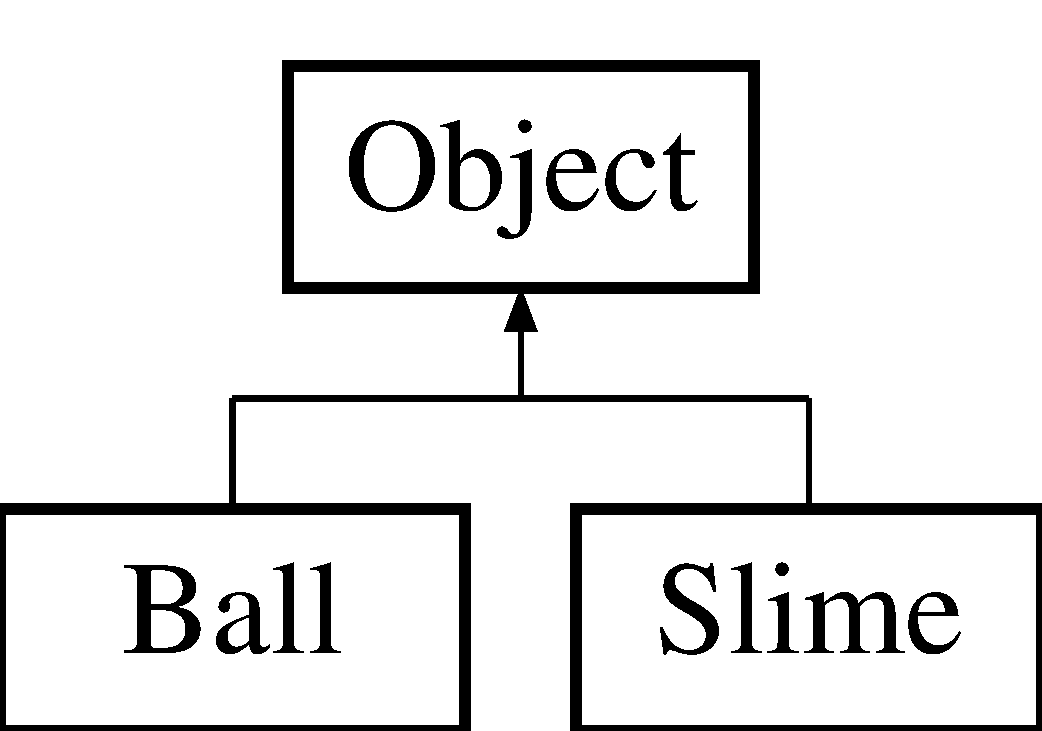
\includegraphics[height=2.000000cm]{classObject}
\end{center}
\end{figure}
\subsection*{Public Member Functions}
\begin{DoxyCompactItemize}
\item 
\hyperlink{classObject_a40860402e64d8008fb42329df7097cdb}{Object} ()
\item 
\hyperlink{classObject_a43ed9b32c482cf0db8bf2d3660feb5f0}{Object} (int, int, int)
\item 
\hyperlink{classObject_ad1af0861169e7b34efc6c86ff971872f}{Object} (int, int, int, char)
\item 
void \hyperlink{classObject_aec33bdfdbb4d45f6060f409a1662134d}{set\-Position} (int, int)
\item 
\hyperlink{structPosition}{Position} \hyperlink{classObject_a3d27536422e7792a3fa7b34ab9862ec4}{get\-Position} ()
\item 
\hypertarget{classObject_ac81f42238b7adaf527b79a5411ca9705}{\hyperlink{structPosition}{Position} {\bfseries get\-Abs\-Position} ()}\label{classObject_ac81f42238b7adaf527b79a5411ca9705}

\item 
\hypertarget{classObject_abbcebc4287c71f92a6f50392bdf9da77}{void {\bfseries set\-Orientation} (int)}\label{classObject_abbcebc4287c71f92a6f50392bdf9da77}

\item 
\hypertarget{classObject_a69d00971216903be3793b082458d0bd9}{int {\bfseries get\-Orientation\-G\-L\-U\-T} ()}\label{classObject_a69d00971216903be3793b082458d0bd9}

\item 
\hypertarget{classObject_a34ad252eded3300ffe5119e768a082a1}{int {\bfseries get\-Orientation} ()}\label{classObject_a34ad252eded3300ffe5119e768a082a1}

\item 
void \hyperlink{classObject_a2143ff47aab9b29336dba6194027edeb}{set\-Radius} (int)
\item 
int \hyperlink{classObject_a82840223125a721f50228530b9b4105f}{get\-Radius} ()
\item 
int \hyperlink{classObject_a60b3199915a0529e3cedd228ae68b913}{collision\-Border} (int, int)
\item 
void \hyperlink{classObject_aaf387599b25880d13058c62091ef739d}{set\-Velocity} (int, int)
\item 
\hypertarget{classObject_ac273a6182758926b972b1e9d73fbf562}{\hyperlink{structVelocity}{Velocity} {\bfseries get\-Velocity} ()}\label{classObject_ac273a6182758926b972b1e9d73fbf562}

\item 
void \hyperlink{classObject_a627ab558ee01d1cb6865ff4f60f5568b}{set\-Color} (char)
\item 
char \hyperlink{classObject_a7d16042d20401814b7d2922ca1023aa3}{get\-Color} ()
\item 
bool \hyperlink{classObject_ab75112940a2a3941b9856529f283e9a8}{collision\-Obstacle} (\hyperlink{classObject}{Object} r)
\item 
int \hyperlink{classObject_aed0e66208e6a5c4595f20e32041917de}{get\-Distance} (\hyperlink{structPosition}{Position})
\item 
\hypertarget{classObject_a5d95415c2e3fe9ab7fdc1a2d2f85c6d7}{void {\bfseries orient\-Towards} (\hyperlink{structPosition}{Position})}\label{classObject_a5d95415c2e3fe9ab7fdc1a2d2f85c6d7}

\item 
int \hyperlink{classObject_a3c70fb123af0439b5d1c916ca74237a8}{angle\-Of} (\hyperlink{structPosition}{Position})
\item 
void \hyperlink{classObject_ac1894a4a885cb94ccd25fb3291599153}{translate} (int)
\end{DoxyCompactItemize}
\subsection*{Public Attributes}
\begin{DoxyCompactItemize}
\item 
\hyperlink{structPosition}{Position} \hyperlink{classObject_ad5b0ba88b937905bd86696917b252b8b}{position}
\item 
\hypertarget{classObject_a9f84fc31e8a08359d432ff7beb146501}{\hyperlink{structVelocity}{Velocity} {\bfseries velocity}}\label{classObject_a9f84fc31e8a08359d432ff7beb146501}

\end{DoxyCompactItemize}
\subsection*{Static Public Attributes}
\begin{DoxyCompactItemize}
\item 
\hypertarget{classObject_aa8fc90771d9d3dce661deb5ee14662a8}{static const int {\bfseries S\-C\-A\-L\-A\-R} = 1000}\label{classObject_aa8fc90771d9d3dce661deb5ee14662a8}

\end{DoxyCompactItemize}
\subsection*{Protected Attributes}
\begin{DoxyCompactItemize}
\item 
\hypertarget{classObject_a6937bdcbc9efbcc6ed7347243819ed77}{char {\bfseries color}}\label{classObject_a6937bdcbc9efbcc6ed7347243819ed77}

\item 
\hypertarget{classObject_abb2dc186dcec09160e6211e84120f0a5}{int {\bfseries radius}}\label{classObject_abb2dc186dcec09160e6211e84120f0a5}

\end{DoxyCompactItemize}


\subsection{Constructor \& Destructor Documentation}
\hypertarget{classObject_a40860402e64d8008fb42329df7097cdb}{\index{Object@{Object}!Object@{Object}}
\index{Object@{Object}!Object@{Object}}
\subsubsection[{Object}]{\setlength{\rightskip}{0pt plus 5cm}Object\-::\-Object (
\begin{DoxyParamCaption}
{}
\end{DoxyParamCaption}
)}}\label{classObject_a40860402e64d8008fb42329df7097cdb}
Default and other constructors

Written on by Alex Wang get\-Distance written by Matt Bullis

Null/default constructor \begin{DoxyAuthor}{Author}
Alex Wang 
\end{DoxyAuthor}

\begin{DoxyParams}{Parameters}
{\em x\-Position} & for x coordinate \\
\hline
{\em y\-Position} & for y coordinate \\
\hline
{\em radius} & for radius, in int \\
\hline
\end{DoxyParams}
\hypertarget{classObject_a43ed9b32c482cf0db8bf2d3660feb5f0}{\index{Object@{Object}!Object@{Object}}
\index{Object@{Object}!Object@{Object}}
\subsubsection[{Object}]{\setlength{\rightskip}{0pt plus 5cm}Object\-::\-Object (
\begin{DoxyParamCaption}
\item[{int}]{x, }
\item[{int}]{y, }
\item[{int}]{r}
\end{DoxyParamCaption}
)}}\label{classObject_a43ed9b32c482cf0db8bf2d3660feb5f0}
Constructor with three passed parameters \begin{DoxyAuthor}{Author}
Alex Wang 
\end{DoxyAuthor}

\begin{DoxyParams}{Parameters}
{\em int} & x for x coordinate \\
\hline
{\em int} & y for y coordinate \\
\hline
{\em int} & r for radius \\
\hline
\end{DoxyParams}
\hypertarget{classObject_ad1af0861169e7b34efc6c86ff971872f}{\index{Object@{Object}!Object@{Object}}
\index{Object@{Object}!Object@{Object}}
\subsubsection[{Object}]{\setlength{\rightskip}{0pt plus 5cm}Object\-::\-Object (
\begin{DoxyParamCaption}
\item[{int}]{x, }
\item[{int}]{y, }
\item[{int}]{r, }
\item[{char}]{c}
\end{DoxyParamCaption}
)}}\label{classObject_ad1af0861169e7b34efc6c86ff971872f}
Constructor with three passed parameters \begin{DoxyAuthor}{Author}
Alex Wang 
\end{DoxyAuthor}

\begin{DoxyParams}{Parameters}
{\em int} & x for x coordinate \\
\hline
{\em int} & y for y coordinate \\
\hline
{\em int} & r for radius \\
\hline
{\em char} & c for color \\
\hline
\end{DoxyParams}


\subsection{Member Function Documentation}
\hypertarget{classObject_a3c70fb123af0439b5d1c916ca74237a8}{\index{Object@{Object}!angle\-Of@{angle\-Of}}
\index{angle\-Of@{angle\-Of}!Object@{Object}}
\subsubsection[{angle\-Of}]{\setlength{\rightskip}{0pt plus 5cm}int Object\-::angle\-Of (
\begin{DoxyParamCaption}
\item[{{\bf Position}}]{p}
\end{DoxyParamCaption}
)}}\label{classObject_a3c70fb123af0439b5d1c916ca74237a8}
This function requires one parameters\-: p. 
\begin{DoxyParams}{Parameters}
{\em p} & the position the objectis located at \\
\hline
\end{DoxyParams}
\begin{DoxyAuthor}{Author}
Matt Bullis 
\end{DoxyAuthor}
\hypertarget{classObject_a60b3199915a0529e3cedd228ae68b913}{\index{Object@{Object}!collision\-Border@{collision\-Border}}
\index{collision\-Border@{collision\-Border}!Object@{Object}}
\subsubsection[{collision\-Border}]{\setlength{\rightskip}{0pt plus 5cm}int Object\-::collision\-Border (
\begin{DoxyParamCaption}
\item[{int}]{x, }
\item[{int}]{y}
\end{DoxyParamCaption}
)}}\label{classObject_a60b3199915a0529e3cedd228ae68b913}
Checks to see if the robot has collided with the border returns an array of four elements each representing a border if there is a collision with the right border, returns 1 if there is a collision with the upper border, returns 2 if there is a collision with the left border, returns 3 if there is a collision with the bottom border, returns 4 
\begin{DoxyParams}{Parameters}
{\em x} & and y are both coordinates of the new position \\
\hline
{\em $\ast$array} & is a array of robot objects containing the robot, obstacles, and the target \\
\hline
\end{DoxyParams}
\begin{DoxyAuthor}{Author}
Aaron Switzer 
\end{DoxyAuthor}
\hypertarget{classObject_ab75112940a2a3941b9856529f283e9a8}{\index{Object@{Object}!collision\-Obstacle@{collision\-Obstacle}}
\index{collision\-Obstacle@{collision\-Obstacle}!Object@{Object}}
\subsubsection[{collision\-Obstacle}]{\setlength{\rightskip}{0pt plus 5cm}bool Object\-::collision\-Obstacle (
\begin{DoxyParamCaption}
\item[{{\bf Object}}]{r}
\end{DoxyParamCaption}
)}}\label{classObject_ab75112940a2a3941b9856529f283e9a8}
returns true if Is object is colliding with another object returns false otherwise 
\begin{DoxyParams}{Parameters}
{\em \hyperlink{classObject}{Object}} & r for object to test collision against \\
\hline
\end{DoxyParams}
\begin{DoxyAuthor}{Author}
Aaron Switzer. 
\end{DoxyAuthor}
\hypertarget{classObject_a7d16042d20401814b7d2922ca1023aa3}{\index{Object@{Object}!get\-Color@{get\-Color}}
\index{get\-Color@{get\-Color}!Object@{Object}}
\subsubsection[{get\-Color}]{\setlength{\rightskip}{0pt plus 5cm}char Object\-::get\-Color (
\begin{DoxyParamCaption}
{}
\end{DoxyParamCaption}
)}}\label{classObject_a7d16042d20401814b7d2922ca1023aa3}
returns color for a given object \begin{DoxyAuthor}{Author}
Alex Wang 
\end{DoxyAuthor}
\hypertarget{classObject_aed0e66208e6a5c4595f20e32041917de}{\index{Object@{Object}!get\-Distance@{get\-Distance}}
\index{get\-Distance@{get\-Distance}!Object@{Object}}
\subsubsection[{get\-Distance}]{\setlength{\rightskip}{0pt plus 5cm}int Object\-::get\-Distance (
\begin{DoxyParamCaption}
\item[{{\bf Position}}]{p}
\end{DoxyParamCaption}
)}}\label{classObject_aed0e66208e6a5c4595f20e32041917de}
returns distance of object and a given position 
\begin{DoxyParams}{Parameters}
{\em \hyperlink{structPosition}{Position}} & p for calculating the distance \\
\hline
\end{DoxyParams}
\begin{DoxyAuthor}{Author}
Matt Bullis 
\end{DoxyAuthor}
\hypertarget{classObject_a3d27536422e7792a3fa7b34ab9862ec4}{\index{Object@{Object}!get\-Position@{get\-Position}}
\index{get\-Position@{get\-Position}!Object@{Object}}
\subsubsection[{get\-Position}]{\setlength{\rightskip}{0pt plus 5cm}{\bf Position} Object\-::get\-Position (
\begin{DoxyParamCaption}
{}
\end{DoxyParamCaption}
)}}\label{classObject_a3d27536422e7792a3fa7b34ab9862ec4}
returns position for a given object \begin{DoxyAuthor}{Author}
Alex Wang 
\end{DoxyAuthor}
\hypertarget{classObject_a82840223125a721f50228530b9b4105f}{\index{Object@{Object}!get\-Radius@{get\-Radius}}
\index{get\-Radius@{get\-Radius}!Object@{Object}}
\subsubsection[{get\-Radius}]{\setlength{\rightskip}{0pt plus 5cm}int Object\-::get\-Radius (
\begin{DoxyParamCaption}
{}
\end{DoxyParamCaption}
)}}\label{classObject_a82840223125a721f50228530b9b4105f}
returns radius for a given object \begin{DoxyAuthor}{Author}
Alex Wang 
\end{DoxyAuthor}
\hypertarget{classObject_a627ab558ee01d1cb6865ff4f60f5568b}{\index{Object@{Object}!set\-Color@{set\-Color}}
\index{set\-Color@{set\-Color}!Object@{Object}}
\subsubsection[{set\-Color}]{\setlength{\rightskip}{0pt plus 5cm}void Object\-::set\-Color (
\begin{DoxyParamCaption}
\item[{char}]{c}
\end{DoxyParamCaption}
)}}\label{classObject_a627ab558ee01d1cb6865ff4f60f5568b}
sets color for a given object \begin{DoxyAuthor}{Author}
Alex Wang 
\end{DoxyAuthor}

\begin{DoxyParams}{Parameters}
{\em char} & c to set color \\
\hline
\end{DoxyParams}
\hypertarget{classObject_aec33bdfdbb4d45f6060f409a1662134d}{\index{Object@{Object}!set\-Position@{set\-Position}}
\index{set\-Position@{set\-Position}!Object@{Object}}
\subsubsection[{set\-Position}]{\setlength{\rightskip}{0pt plus 5cm}void Object\-::set\-Position (
\begin{DoxyParamCaption}
\item[{int}]{x, }
\item[{int}]{y}
\end{DoxyParamCaption}
)}}\label{classObject_aec33bdfdbb4d45f6060f409a1662134d}
Methods for functionality

sets position for a given object for x and y parameters \begin{DoxyAuthor}{Author}
Alex Wang 
\end{DoxyAuthor}

\begin{DoxyParams}{Parameters}
{\em int} & x to set x coordinate \\
\hline
{\em int} & y to set y coordinate \\
\hline
\end{DoxyParams}
\hypertarget{classObject_a2143ff47aab9b29336dba6194027edeb}{\index{Object@{Object}!set\-Radius@{set\-Radius}}
\index{set\-Radius@{set\-Radius}!Object@{Object}}
\subsubsection[{set\-Radius}]{\setlength{\rightskip}{0pt plus 5cm}void Object\-::set\-Radius (
\begin{DoxyParamCaption}
\item[{int}]{r}
\end{DoxyParamCaption}
)}}\label{classObject_a2143ff47aab9b29336dba6194027edeb}
sets radius for a given object \begin{DoxyAuthor}{Author}
Alex Wang 
\end{DoxyAuthor}

\begin{DoxyParams}{Parameters}
{\em int} & r to set radius \\
\hline
\end{DoxyParams}
\hypertarget{classObject_aaf387599b25880d13058c62091ef739d}{\index{Object@{Object}!set\-Velocity@{set\-Velocity}}
\index{set\-Velocity@{set\-Velocity}!Object@{Object}}
\subsubsection[{set\-Velocity}]{\setlength{\rightskip}{0pt plus 5cm}void Object\-::set\-Velocity (
\begin{DoxyParamCaption}
\item[{int}]{xv, }
\item[{int}]{yv}
\end{DoxyParamCaption}
)}}\label{classObject_aaf387599b25880d13058c62091ef739d}
sets the speed of an object 
\begin{DoxyParams}{Parameters}
{\em int} & speed that is the speed variable \\
\hline
\end{DoxyParams}
\begin{DoxyAuthor}{Author}
Alex Wang 
\end{DoxyAuthor}
\hypertarget{classObject_ac1894a4a885cb94ccd25fb3291599153}{\index{Object@{Object}!translate@{translate}}
\index{translate@{translate}!Object@{Object}}
\subsubsection[{translate}]{\setlength{\rightskip}{0pt plus 5cm}void Object\-::translate (
\begin{DoxyParamCaption}
\item[{int}]{pixels}
\end{DoxyParamCaption}
)}}\label{classObject_ac1894a4a885cb94ccd25fb3291599153}
This function requires one parameters\-: pixels. 
\begin{DoxyParams}{Parameters}
{\em pixels} & the distance to be travelled in pixels \\
\hline
\end{DoxyParams}
\begin{DoxyAuthor}{Author}
Matt Bullis 
\end{DoxyAuthor}


\subsection{Member Data Documentation}
\hypertarget{classObject_ad5b0ba88b937905bd86696917b252b8b}{\index{Object@{Object}!position@{position}}
\index{position@{position}!Object@{Object}}
\subsubsection[{position}]{\setlength{\rightskip}{0pt plus 5cm}{\bf Position} Object\-::position}}\label{classObject_ad5b0ba88b937905bd86696917b252b8b}
Variables for position and radius and color 

The documentation for this class was generated from the following files\-:\begin{DoxyCompactItemize}
\item 
Object.\-h\item 
Object.\-cpp\end{DoxyCompactItemize}

\hypertarget{structPosition}{\section{Position Struct Reference}
\label{structPosition}\index{Position@{Position}}
}


{\ttfamily \#include $<$Object.\-h$>$}

\subsection*{Public Attributes}
\begin{DoxyCompactItemize}
\item 
\hypertarget{structPosition_a98b626e4dc812dc82b59b830f0c11e9c}{int {\bfseries x\-Position}}\label{structPosition_a98b626e4dc812dc82b59b830f0c11e9c}

\item 
\hypertarget{structPosition_af49c9e30e516f34e6ec5458b171208d0}{int {\bfseries y\-Position}}\label{structPosition_af49c9e30e516f34e6ec5458b171208d0}

\end{DoxyCompactItemize}


\subsection{Detailed Description}
Written by Alex Wang

\hyperlink{classObject}{Object} class, main class

New data structure used for coordinates 

The documentation for this struct was generated from the following file\-:\begin{DoxyCompactItemize}
\item 
Object.\-h\end{DoxyCompactItemize}

\hypertarget{classRenderEnv}{\section{Render\-Env Class Reference}
\label{classRenderEnv}\index{Render\-Env@{Render\-Env}}
}


{\ttfamily \#include $<$Render\-Env.\-h$>$}

\subsection*{Public Member Functions}
\begin{DoxyCompactItemize}
\item 
void \hyperlink{classRenderEnv_ad3b1c8841f9d4b7e9c140bf2289b0af1}{start\-Simulation} ()
\end{DoxyCompactItemize}


\subsection{Detailed Description}
\hyperlink{classRenderEnv}{Render\-Env} class written by Alex Wang and Arun Parthiban 

\subsection{Member Function Documentation}
\hypertarget{classRenderEnv_ad3b1c8841f9d4b7e9c140bf2289b0af1}{\index{Render\-Env@{Render\-Env}!start\-Simulation@{start\-Simulation}}
\index{start\-Simulation@{start\-Simulation}!RenderEnv@{Render\-Env}}
\subsubsection[{start\-Simulation}]{\setlength{\rightskip}{0pt plus 5cm}void Render\-Env\-::start\-Simulation (
\begin{DoxyParamCaption}
{}
\end{DoxyParamCaption}
)}}\label{classRenderEnv_ad3b1c8841f9d4b7e9c140bf2289b0af1}
This function starts the game. By Placing the Slimes and ball in the environment. \begin{DoxyAuthor}{Author}
Matthew Bullis 
\end{DoxyAuthor}


The documentation for this class was generated from the following files\-:\begin{DoxyCompactItemize}
\item 
Render\-Env.\-h\item 
Render\-Env.\-cpp\end{DoxyCompactItemize}

\hypertarget{classSlime}{\section{Slime Class Reference}
\label{classSlime}\index{Slime@{Slime}}
}
Inheritance diagram for Slime\-:\begin{figure}[H]
\begin{center}
\leavevmode
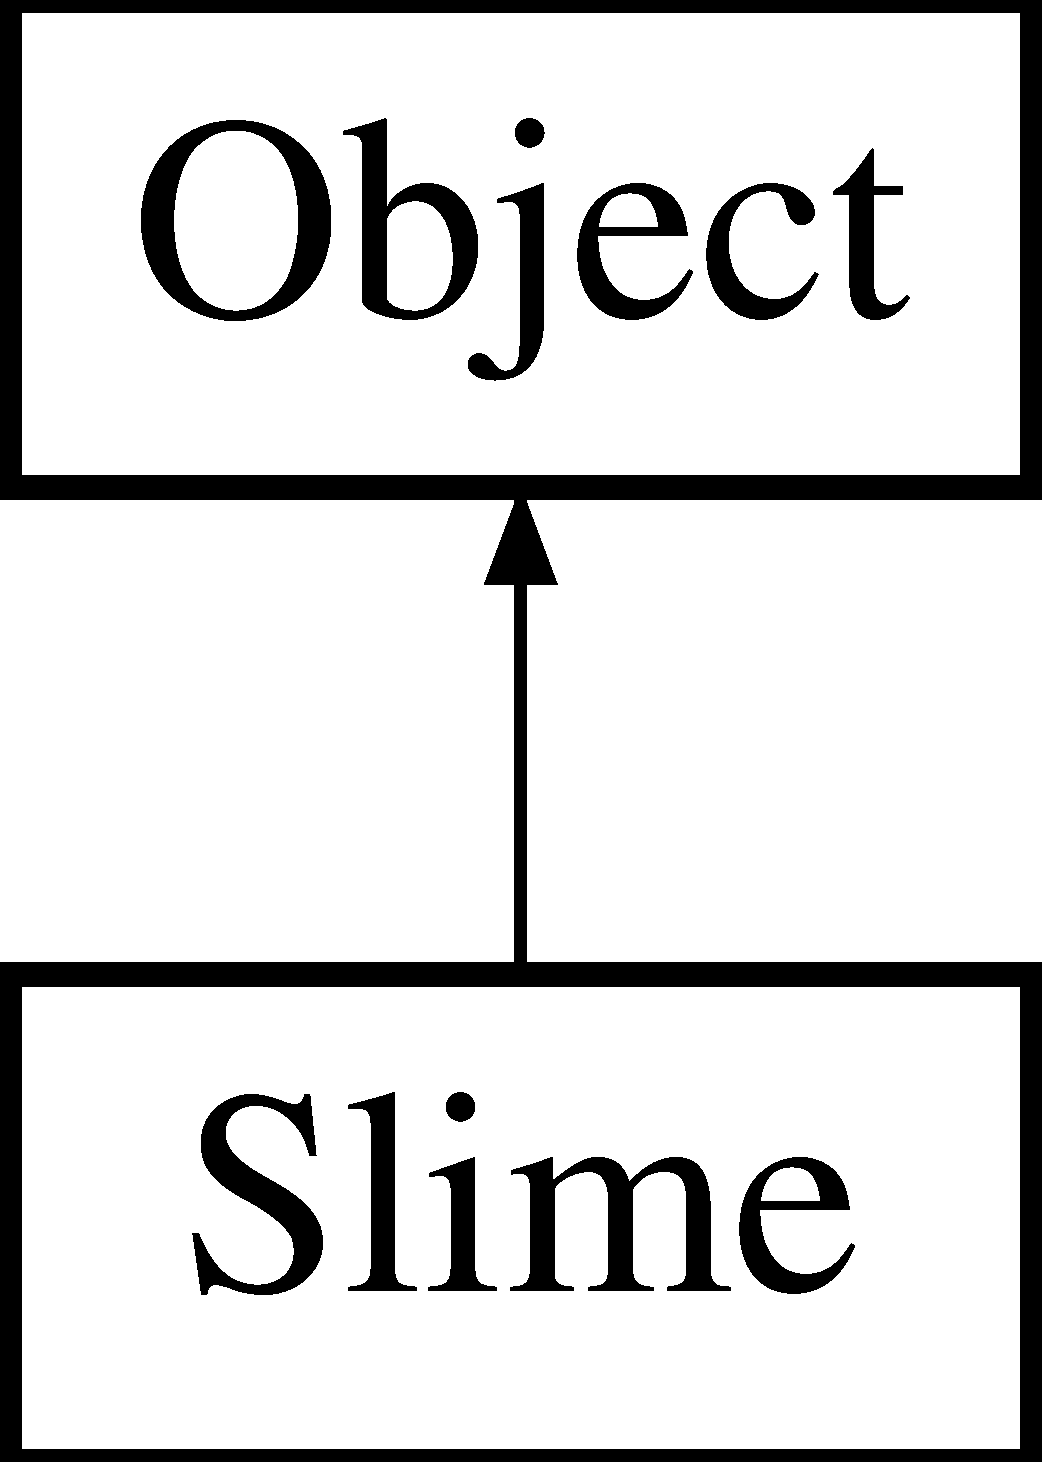
\includegraphics[height=2.000000cm]{classSlime}
\end{center}
\end{figure}
\subsection*{Public Member Functions}
\begin{DoxyCompactItemize}
\item 
\hyperlink{classSlime_a311bc6c56df2c1f7660a08634e560db6}{Slime} ()
\item 
\hyperlink{classSlime_ae3f09154eb9ffeb1e3f40914f85e7fb8}{Slime} (int, int, char)
\item 
void \hyperlink{classSlime_a369c16e49e7cbc425c7486d9e914ecc5}{move} (int)
\item 
void \hyperlink{classSlime_a825cc65a1acef3382eb986567b9f9639}{set\-Input} (int)
\item 
void \hyperlink{classSlime_a8cb4328663278acf60995d2d47894f14}{move\-To} (\hyperlink{structPosition}{Position})
\item 
void \hyperlink{classSlime_a3f7637800c973e4e8fbdf899e911c59e}{play\-Defense} (\hyperlink{structPosition}{Position}, \hyperlink{structPosition}{Position}, \hyperlink{structVelocity}{Velocity})
\item 
void \hyperlink{classSlime_af50875e65a9a9a1ce4880ba4b4864436}{return\-Ball} (\hyperlink{structPosition}{Position}, \hyperlink{structPosition}{Position}, \hyperlink{structVelocity}{Velocity})
\end{DoxyCompactItemize}
\subsection*{Static Public Attributes}
\begin{DoxyCompactItemize}
\item 
\hypertarget{classSlime_a33c70f396f273db5c1bd716a7f520bb2}{static const int {\bfseries move\-Error\-Acceptance} = 2}\label{classSlime_a33c70f396f273db5c1bd716a7f520bb2}

\item 
\hypertarget{classSlime_a5b95a92ca5e1c3f3b93522f66fbc2668}{static const int {\bfseries screen\-Size} = 800}\label{classSlime_a5b95a92ca5e1c3f3b93522f66fbc2668}

\item 
\hypertarget{classSlime_a90330dacbc5c177c82a054da6505cd2c}{static const int {\bfseries move\-Speed} = 300}\label{classSlime_a90330dacbc5c177c82a054da6505cd2c}

\item 
\hypertarget{classSlime_a35adc59a855a3e0e5857889a559e7aa9}{static const int {\bfseries jump\-Speed} = 600}\label{classSlime_a35adc59a855a3e0e5857889a559e7aa9}

\end{DoxyCompactItemize}
\subsection*{Additional Inherited Members}


\subsection{Constructor \& Destructor Documentation}
\hypertarget{classSlime_a311bc6c56df2c1f7660a08634e560db6}{\index{Slime@{Slime}!Slime@{Slime}}
\index{Slime@{Slime}!Slime@{Slime}}
\subsubsection[{Slime}]{\setlength{\rightskip}{0pt plus 5cm}Slime\-::\-Slime (
\begin{DoxyParamCaption}
{}
\end{DoxyParamCaption}
)}}\label{classSlime_a311bc6c56df2c1f7660a08634e560db6}
default constructor initializes all variables \begin{DoxyAuthor}{Author}
Matthew Bullis 
\end{DoxyAuthor}
\hypertarget{classSlime_ae3f09154eb9ffeb1e3f40914f85e7fb8}{\index{Slime@{Slime}!Slime@{Slime}}
\index{Slime@{Slime}!Slime@{Slime}}
\subsubsection[{Slime}]{\setlength{\rightskip}{0pt plus 5cm}Slime\-::\-Slime (
\begin{DoxyParamCaption}
\item[{int}]{xpos, }
\item[{int}]{ypos, }
\item[{char}]{c}
\end{DoxyParamCaption}
)}}\label{classSlime_ae3f09154eb9ffeb1e3f40914f85e7fb8}
Constructor with three passed parameters \begin{DoxyAuthor}{Author}
Matthew Bullis 
\end{DoxyAuthor}

\begin{DoxyParams}{Parameters}
{\em int} & xpos for x coordinate \\
\hline
{\em int} & ypos for y coordinate \\
\hline
{\em char} & c for color \\
\hline
\end{DoxyParams}


\subsection{Member Function Documentation}
\hypertarget{classSlime_a369c16e49e7cbc425c7486d9e914ecc5}{\index{Slime@{Slime}!move@{move}}
\index{move@{move}!Slime@{Slime}}
\subsubsection[{move}]{\setlength{\rightskip}{0pt plus 5cm}void Slime\-::move (
\begin{DoxyParamCaption}
\item[{int}]{time}
\end{DoxyParamCaption}
)}}\label{classSlime_a369c16e49e7cbc425c7486d9e914ecc5}
Updates the position based on the current input 
\begin{DoxyParams}{Parameters}
{\em int} & time for elapsed time. \\
\hline
\end{DoxyParams}
\begin{DoxyAuthor}{Author}
Matthew Bullis 
\end{DoxyAuthor}
\hypertarget{classSlime_a8cb4328663278acf60995d2d47894f14}{\index{Slime@{Slime}!move\-To@{move\-To}}
\index{move\-To@{move\-To}!Slime@{Slime}}
\subsubsection[{move\-To}]{\setlength{\rightskip}{0pt plus 5cm}void Slime\-::move\-To (
\begin{DoxyParamCaption}
\item[{{\bf Position}}]{p}
\end{DoxyParamCaption}
)}}\label{classSlime_a8cb4328663278acf60995d2d47894f14}
When single player move\-To is the A\-I responsible for moveing to position p 
\begin{DoxyParams}{Parameters}
{\em \hyperlink{structPosition}{Position}} & p is the destination. \\
\hline
\end{DoxyParams}
\begin{DoxyAuthor}{Author}
Matthew Bullis 
\end{DoxyAuthor}
\hypertarget{classSlime_a3f7637800c973e4e8fbdf899e911c59e}{\index{Slime@{Slime}!play\-Defense@{play\-Defense}}
\index{play\-Defense@{play\-Defense}!Slime@{Slime}}
\subsubsection[{play\-Defense}]{\setlength{\rightskip}{0pt plus 5cm}void Slime\-::play\-Defense (
\begin{DoxyParamCaption}
\item[{{\bf Position}}]{p, }
\item[{{\bf Position}}]{s, }
\item[{{\bf Velocity}}]{V}
\end{DoxyParamCaption}
)}}\label{classSlime_a3f7637800c973e4e8fbdf899e911c59e}
When single player play\-Defense is the A\-I responsible for deciding how to act when the ball is not in p2's court 
\begin{DoxyParams}{Parameters}
{\em \hyperlink{structPosition}{Position}} & p is where the ball with hit the ground. \\
\hline
{\em \hyperlink{structPosition}{Position}} & s is the enemy slime's current position \\
\hline
{\em \hyperlink{structVelocity}{Velocity}} & V is the velocity of the ball \\
\hline
\end{DoxyParams}
\begin{DoxyAuthor}{Author}
Matthew Bullis 
\end{DoxyAuthor}
\hypertarget{classSlime_af50875e65a9a9a1ce4880ba4b4864436}{\index{Slime@{Slime}!return\-Ball@{return\-Ball}}
\index{return\-Ball@{return\-Ball}!Slime@{Slime}}
\subsubsection[{return\-Ball}]{\setlength{\rightskip}{0pt plus 5cm}void Slime\-::return\-Ball (
\begin{DoxyParamCaption}
\item[{{\bf Position}}]{p, }
\item[{{\bf Position}}]{s, }
\item[{{\bf Velocity}}]{V}
\end{DoxyParamCaption}
)}}\label{classSlime_af50875e65a9a9a1ce4880ba4b4864436}
When single player return\-Ball is the A\-I responsible for deciding how hard to hit the ball 
\begin{DoxyParams}{Parameters}
{\em \hyperlink{structPosition}{Position}} & p is where the ball with hit the ground. \\
\hline
{\em \hyperlink{structPosition}{Position}} & s is the enemy slime's current position \\
\hline
{\em \hyperlink{structVelocity}{Velocity}} & V is the velocity of the ball \\
\hline
\end{DoxyParams}
\begin{DoxyAuthor}{Author}
Matthew Bullis 
\end{DoxyAuthor}
\hypertarget{classSlime_a825cc65a1acef3382eb986567b9f9639}{\index{Slime@{Slime}!set\-Input@{set\-Input}}
\index{set\-Input@{set\-Input}!Slime@{Slime}}
\subsubsection[{set\-Input}]{\setlength{\rightskip}{0pt plus 5cm}void Slime\-::set\-Input (
\begin{DoxyParamCaption}
\item[{int}]{i}
\end{DoxyParamCaption}
)}}\label{classSlime_a825cc65a1acef3382eb986567b9f9639}
Updates the slimes travel direction based on the latest 
\begin{DoxyParams}{Parameters}
{\em int} & i for last input \\
\hline
\end{DoxyParams}
\begin{DoxyAuthor}{Author}
Matthew Bullis 
\end{DoxyAuthor}


The documentation for this class was generated from the following files\-:\begin{DoxyCompactItemize}
\item 
Slime.\-h\item 
Slime.\-cpp\end{DoxyCompactItemize}

\hypertarget{structVelocity}{\section{Velocity Struct Reference}
\label{structVelocity}\index{Velocity@{Velocity}}
}
\subsection*{Public Attributes}
\begin{DoxyCompactItemize}
\item 
\hypertarget{structVelocity_a87d82f672105324e6c5a93a763f6d686}{int {\bfseries x\-Vel}}\label{structVelocity_a87d82f672105324e6c5a93a763f6d686}

\item 
\hypertarget{structVelocity_a400c85cbd1669348aca25afe0ae95883}{int {\bfseries y\-Vel}}\label{structVelocity_a400c85cbd1669348aca25afe0ae95883}

\end{DoxyCompactItemize}


The documentation for this struct was generated from the following file\-:\begin{DoxyCompactItemize}
\item 
Object.\-h\end{DoxyCompactItemize}

\chapter{File Documentation}
\hypertarget{drawing_8cpp}{\section{drawing.\-cpp File Reference}
\label{drawing_8cpp}\index{drawing.\-cpp@{drawing.\-cpp}}
}
{\ttfamily \#include $<$math.\-h$>$}\\*
{\ttfamily \#include \char`\"{}Object.\-h\char`\"{}}\\*
{\ttfamily \#include \char`\"{}drawing.\-h\char`\"{}}\\*
{\ttfamily \#include $<$G\-L/glut.\-h$>$}\\*
{\ttfamily \#include $<$G\-L/glu.\-h$>$}\\*
{\ttfamily \#include $<$G\-L/glui.\-h$>$}\\*
{\ttfamily \#include $<$cstdlib$>$}\\*
{\ttfamily \#include $<$iostream$>$}\\*
{\ttfamily \#include $<$vector$>$}\\*
{\ttfamily \#include \char`\"{}environment.\-h\char`\"{}}\\*
\subsection*{Macros}
\begin{DoxyCompactItemize}
\item 
\#define \hyperlink{drawing_8cpp_a598a3330b3c21701223ee0ca14316eca}{P\-I}~3.\-14f
\end{DoxyCompactItemize}
\subsection*{Functions}
\begin{DoxyCompactItemize}
\item 
\hypertarget{drawing_8cpp_a1be686b4203466efcfc18ada8b9b2853}{void {\bfseries menu} (int id)}\label{drawing_8cpp_a1be686b4203466efcfc18ada8b9b2853}

\item 
\hypertarget{drawing_8cpp_a1bc781d5d2cb4613bb6157f8fc012d96}{void {\bfseries set\-Color} (char c)}\label{drawing_8cpp_a1bc781d5d2cb4613bb6157f8fc012d96}

\item 
void \hyperlink{drawing_8cpp_afcdf404cece45fdc9daffe1a0b48974c}{draw\-Net} (int xpos, int height)
\item 
\hypertarget{drawing_8cpp_a2b66f507378132a69eb038d1f27097bd}{void {\bfseries draw\-Slime} (\hyperlink{classSlime}{Slime} shaddy)}\label{drawing_8cpp_a2b66f507378132a69eb038d1f27097bd}

\item 
void \hyperlink{drawing_8cpp_a914ad5a726418ab9b69b0071718f7ce8}{draw\-Ball} (\hyperlink{classBall}{Ball} b)
\item 
void \hyperlink{drawing_8cpp_a4ea013001a5fb47853d0fab8f8de35cd}{display} (void)
\item 
void \hyperlink{drawing_8cpp_afd41946fdeaf7f653c07d140d70a11b7}{freeze\-Display} (void)
\item 
void \hyperlink{drawing_8cpp_a2313c6c5995e9023c607833af1bd4db5}{un\-Freeze} (void)
\item 
void \hyperlink{drawing_8cpp_adceba7dd8273e91208ca6e7f3d3db90f}{freeze} (void)
\item 
void \hyperlink{drawing_8cpp_a6819355374dd277347abd7c4235f0cd7}{reshape} (int width, int height)
\item 
void \hyperlink{drawing_8cpp_a01131b63acf241e9db91704d89ce15d2}{idle} (void)
\item 
void \hyperlink{drawing_8cpp_a8543b063f342565856b74f22bd583453}{set\-Single} (void)
\item 
void \hyperlink{drawing_8cpp_abef157af3d5bfae1eeb0fd1464b5298c}{set\-Multi} (void)
\item 
int \hyperlink{drawing_8cpp_aa3031dd280646724740dc9b0092906cc}{run\-Glut} ()
\item 
\hypertarget{drawing_8cpp_a921b29eb9802cb833818c43c4b17cb37}{void {\bfseries process\-Normal\-Keys} (unsigned char key, int x, int y)}\label{drawing_8cpp_a921b29eb9802cb833818c43c4b17cb37}

\item 
\hypertarget{drawing_8cpp_a78f6ec96acbb8156cd856466cf3848e5}{void {\bfseries key\-Up} (unsigned char key, int x, int y)}\label{drawing_8cpp_a78f6ec96acbb8156cd856466cf3848e5}

\item 
\hypertarget{drawing_8cpp_a64f0952205a2d490b6b5f14b806e3eb7}{void {\bfseries process\-Special\-Keys} (int key, int x, int y)}\label{drawing_8cpp_a64f0952205a2d490b6b5f14b806e3eb7}

\item 
\hypertarget{drawing_8cpp_a529355f27542469edae78a503c5103a9}{void {\bfseries key\-Special\-Up} (int key, int x, int y)}\label{drawing_8cpp_a529355f27542469edae78a503c5103a9}

\end{DoxyCompactItemize}
\subsection*{Variables}
\begin{DoxyCompactItemize}
\item 
\hyperlink{classenvironment}{environment} \hyperlink{drawing_8cpp_a47490e9bb403616123bb09400e317ac7}{env}
\item 
\hypertarget{drawing_8cpp_a65ba7a0b8164c01b33d92b9ab0f2af03}{int {\bfseries window}}\label{drawing_8cpp_a65ba7a0b8164c01b33d92b9ab0f2af03}

\item 
\hypertarget{drawing_8cpp_aaa2bba9b04515c5bbf5c04d20f672b12}{int {\bfseries previous\-Time}}\label{drawing_8cpp_aaa2bba9b04515c5bbf5c04d20f672b12}

\item 
\hypertarget{drawing_8cpp_a73ab6b9ae8c97849c3323ef4fe822ad3}{int {\bfseries current\-Time}}\label{drawing_8cpp_a73ab6b9ae8c97849c3323ef4fe822ad3}

\item 
\hypertarget{drawing_8cpp_aeda1fc5c02ff3c855b3b145567058cb9}{int {\bfseries elapsed\-Time}}\label{drawing_8cpp_aeda1fc5c02ff3c855b3b145567058cb9}

\end{DoxyCompactItemize}


\subsection{Macro Definition Documentation}
\hypertarget{drawing_8cpp_a598a3330b3c21701223ee0ca14316eca}{\index{drawing.\-cpp@{drawing.\-cpp}!P\-I@{P\-I}}
\index{P\-I@{P\-I}!drawing.cpp@{drawing.\-cpp}}
\subsubsection[{P\-I}]{\setlength{\rightskip}{0pt plus 5cm}\#define P\-I~3.\-14f}}\label{drawing_8cpp_a598a3330b3c21701223ee0ca14316eca}
Majority of work done by Arun Parthiban Glui methods and menu written by Alex Wang Various edits and fixes done by Aaron Switzer 

\subsection{Function Documentation}
\hypertarget{drawing_8cpp_a4ea013001a5fb47853d0fab8f8de35cd}{\index{drawing.\-cpp@{drawing.\-cpp}!display@{display}}
\index{display@{display}!drawing.cpp@{drawing.\-cpp}}
\subsubsection[{display}]{\setlength{\rightskip}{0pt plus 5cm}void display (
\begin{DoxyParamCaption}
\item[{void}]{}
\end{DoxyParamCaption}
)}}\label{drawing_8cpp_a4ea013001a5fb47853d0fab8f8de35cd}
This function is called to update the display How it works is the elapsed time is calculated each loop and passed into our \hyperlink{classenvironment_acbd5c1e053c91847f7605cd8b29e7a10}{environment.\-update} method \begin{DoxyAuthor}{Author}
Arun Parthiban 

Aaron Switzer 

Alex Wang 
\end{DoxyAuthor}
\hypertarget{drawing_8cpp_a914ad5a726418ab9b69b0071718f7ce8}{\index{drawing.\-cpp@{drawing.\-cpp}!draw\-Ball@{draw\-Ball}}
\index{draw\-Ball@{draw\-Ball}!drawing.cpp@{drawing.\-cpp}}
\subsubsection[{draw\-Ball}]{\setlength{\rightskip}{0pt plus 5cm}void draw\-Ball (
\begin{DoxyParamCaption}
\item[{{\bf Ball}}]{b}
\end{DoxyParamCaption}
)}}\label{drawing_8cpp_a914ad5a726418ab9b69b0071718f7ce8}
This function draws a light on the display 
\begin{DoxyParams}{Parameters}
{\em a} & is a light \\
\hline
\end{DoxyParams}
\begin{DoxyAuthor}{Author}
Alex Wang 
\end{DoxyAuthor}
\hypertarget{drawing_8cpp_afcdf404cece45fdc9daffe1a0b48974c}{\index{drawing.\-cpp@{drawing.\-cpp}!draw\-Net@{draw\-Net}}
\index{draw\-Net@{draw\-Net}!drawing.cpp@{drawing.\-cpp}}
\subsubsection[{draw\-Net}]{\setlength{\rightskip}{0pt plus 5cm}void draw\-Net (
\begin{DoxyParamCaption}
\item[{int}]{xpos, }
\item[{int}]{height}
\end{DoxyParamCaption}
)}}\label{drawing_8cpp_afcdf404cece45fdc9daffe1a0b48974c}
This function draws a robot on the display 
\begin{DoxyParams}{Parameters}
{\em robot} & is a Robot \\
\hline
\end{DoxyParams}
\begin{DoxyAuthor}{Author}
Arun Parthiban 
\end{DoxyAuthor}
\hypertarget{drawing_8cpp_adceba7dd8273e91208ca6e7f3d3db90f}{\index{drawing.\-cpp@{drawing.\-cpp}!freeze@{freeze}}
\index{freeze@{freeze}!drawing.cpp@{drawing.\-cpp}}
\subsubsection[{freeze}]{\setlength{\rightskip}{0pt plus 5cm}void freeze (
\begin{DoxyParamCaption}
\item[{void}]{}
\end{DoxyParamCaption}
)}}\label{drawing_8cpp_adceba7dd8273e91208ca6e7f3d3db90f}
This function freezes the display It works by passing the freeze\-Display function into glut\-Display\-Func all time varaibles are also updated every call, as robots will jump without \begin{DoxyAuthor}{Author}
Alex Wang 
\end{DoxyAuthor}
\hypertarget{drawing_8cpp_afd41946fdeaf7f653c07d140d70a11b7}{\index{drawing.\-cpp@{drawing.\-cpp}!freeze\-Display@{freeze\-Display}}
\index{freeze\-Display@{freeze\-Display}!drawing.cpp@{drawing.\-cpp}}
\subsubsection[{freeze\-Display}]{\setlength{\rightskip}{0pt plus 5cm}void freeze\-Display (
\begin{DoxyParamCaption}
\item[{void}]{}
\end{DoxyParamCaption}
)}}\label{drawing_8cpp_afd41946fdeaf7f653c07d140d70a11b7}
This function is called to freeze the dispay, so no objects are moving how it works is 0 is passed in to our environment update function \begin{DoxyAuthor}{Author}
Alex Wang 
\end{DoxyAuthor}
\hypertarget{drawing_8cpp_a01131b63acf241e9db91704d89ce15d2}{\index{drawing.\-cpp@{drawing.\-cpp}!idle@{idle}}
\index{idle@{idle}!drawing.cpp@{drawing.\-cpp}}
\subsubsection[{idle}]{\setlength{\rightskip}{0pt plus 5cm}void idle (
\begin{DoxyParamCaption}
\item[{void}]{}
\end{DoxyParamCaption}
)}}\label{drawing_8cpp_a01131b63acf241e9db91704d89ce15d2}
Idle fuction called by glut No parameters taken \begin{DoxyAuthor}{Author}
Alex Wang 
\end{DoxyAuthor}
\hypertarget{drawing_8cpp_a6819355374dd277347abd7c4235f0cd7}{\index{drawing.\-cpp@{drawing.\-cpp}!reshape@{reshape}}
\index{reshape@{reshape}!drawing.cpp@{drawing.\-cpp}}
\subsubsection[{reshape}]{\setlength{\rightskip}{0pt plus 5cm}void reshape (
\begin{DoxyParamCaption}
\item[{int}]{width, }
\item[{int}]{height}
\end{DoxyParamCaption}
)}}\label{drawing_8cpp_a6819355374dd277347abd7c4235f0cd7}
Reshapes the glut displayed window 
\begin{DoxyParams}{Parameters}
{\em width} & represents window width \\
\hline
{\em height} & represents window height \\
\hline
\end{DoxyParams}
\begin{DoxyAuthor}{Author}
Arun Parthiban 
\end{DoxyAuthor}
\hypertarget{drawing_8cpp_aa3031dd280646724740dc9b0092906cc}{\index{drawing.\-cpp@{drawing.\-cpp}!run\-Glut@{run\-Glut}}
\index{run\-Glut@{run\-Glut}!drawing.cpp@{drawing.\-cpp}}
\subsubsection[{run\-Glut}]{\setlength{\rightskip}{0pt plus 5cm}int run\-Glut (
\begin{DoxyParamCaption}
{}
\end{DoxyParamCaption}
)}}\label{drawing_8cpp_aa3031dd280646724740dc9b0092906cc}
Drawing class written by Arun, with implementation from Alex and Aaron \hypertarget{drawing_8cpp_abef157af3d5bfae1eeb0fd1464b5298c}{\index{drawing.\-cpp@{drawing.\-cpp}!set\-Multi@{set\-Multi}}
\index{set\-Multi@{set\-Multi}!drawing.cpp@{drawing.\-cpp}}
\subsubsection[{set\-Multi}]{\setlength{\rightskip}{0pt plus 5cm}void set\-Multi (
\begin{DoxyParamCaption}
\item[{void}]{}
\end{DoxyParamCaption}
)}}\label{drawing_8cpp_abef157af3d5bfae1eeb0fd1464b5298c}
This function sets the game to multiplayer It works by changing the environment's multiplayer variable to true \begin{DoxyAuthor}{Author}
Matthew Bullis 
\end{DoxyAuthor}
\hypertarget{drawing_8cpp_a8543b063f342565856b74f22bd583453}{\index{drawing.\-cpp@{drawing.\-cpp}!set\-Single@{set\-Single}}
\index{set\-Single@{set\-Single}!drawing.cpp@{drawing.\-cpp}}
\subsubsection[{set\-Single}]{\setlength{\rightskip}{0pt plus 5cm}void set\-Single (
\begin{DoxyParamCaption}
\item[{void}]{}
\end{DoxyParamCaption}
)}}\label{drawing_8cpp_a8543b063f342565856b74f22bd583453}
Call this function to create the glut display a submenu is also created using G\-L\-U\-I funcitonality includes four buttons\-: quit, pause, resume, and start When a button is clicked, the function that is mapped to it is called \begin{DoxyAuthor}{Author}
Alex Wang 

Arun Parthiban
\end{DoxyAuthor}
This function sets the game to single player It works by changing the environment's multiplayer variable to false \begin{DoxyAuthor}{Author}
Matthew Bullis 
\end{DoxyAuthor}
\hypertarget{drawing_8cpp_a2313c6c5995e9023c607833af1bd4db5}{\index{drawing.\-cpp@{drawing.\-cpp}!un\-Freeze@{un\-Freeze}}
\index{un\-Freeze@{un\-Freeze}!drawing.cpp@{drawing.\-cpp}}
\subsubsection[{un\-Freeze}]{\setlength{\rightskip}{0pt plus 5cm}void un\-Freeze (
\begin{DoxyParamCaption}
\item[{void}]{}
\end{DoxyParamCaption}
)}}\label{drawing_8cpp_a2313c6c5995e9023c607833af1bd4db5}
This function unfreezes the display It works by passing the display function into glut\-Display\-Func all time varaibles are also updated every call, as robots will jump without \begin{DoxyAuthor}{Author}
Alex Wang 
\end{DoxyAuthor}


\subsection{Variable Documentation}
\hypertarget{drawing_8cpp_a47490e9bb403616123bb09400e317ac7}{\index{drawing.\-cpp@{drawing.\-cpp}!env@{env}}
\index{env@{env}!drawing.cpp@{drawing.\-cpp}}
\subsubsection[{env}]{\setlength{\rightskip}{0pt plus 5cm}{\bf environment} env}}\label{drawing_8cpp_a47490e9bb403616123bb09400e317ac7}
\hyperlink{classRenderEnv}{Render\-Env} written by Alex Wang and Arun Parthiban 
%--- End generated contents ---

% Index
\newpage
\phantomsection
\addcontentsline{toc}{chapter}{Index}
\printindex

\end{document}
